\section{PRZEGLĄD ISTNIEJĄCYCH ROZWIĄZAŃ}

\subsection{Wordpress}

Wordpres to najbardziej popularny CMS. Ten system został napisany z myślą o
prezentowaniu treści w formie strony HTML. Wordpress jest napisany w języku PHP
i do działania wymaga zainstalowania serwera HTTP oraz interpretera PHP.
Pierwsze wydanie systemu miało miejsce w roku 2003 i od tamtej pory system jest
ciągle rozwijany.

Modele w systemie CMS to typy danych, którymi można zarządzać. Domyślnym
modelem, w systemie Wordpress jest wpis w blogu. Zawiera między innymi tytuł,
tekst wpisu i datę publikacji. Interfejs tworzenia nowego postu został
przedstawiony na rysunku \ref{wordpressNewPost}. Wordpress pozwala na
definiowanie własnych modeli, ale nie jest to wspierane w domyślnym panelu
administratora. Do stworzenia nowego typu danych, wymagane jest wywołanie
funkcji PHP udostępnionej przez Wordpress, do której nie ma domyślnie interfejsu
użytkownika. Polecanym przez twórców sposobem tworzenia nowych typów danych jest
zainstalowanie wtyczki, która implementuje taki interfejs
\cite{WordpressCustomType}.

\begin{figure}[h]
    \centering
    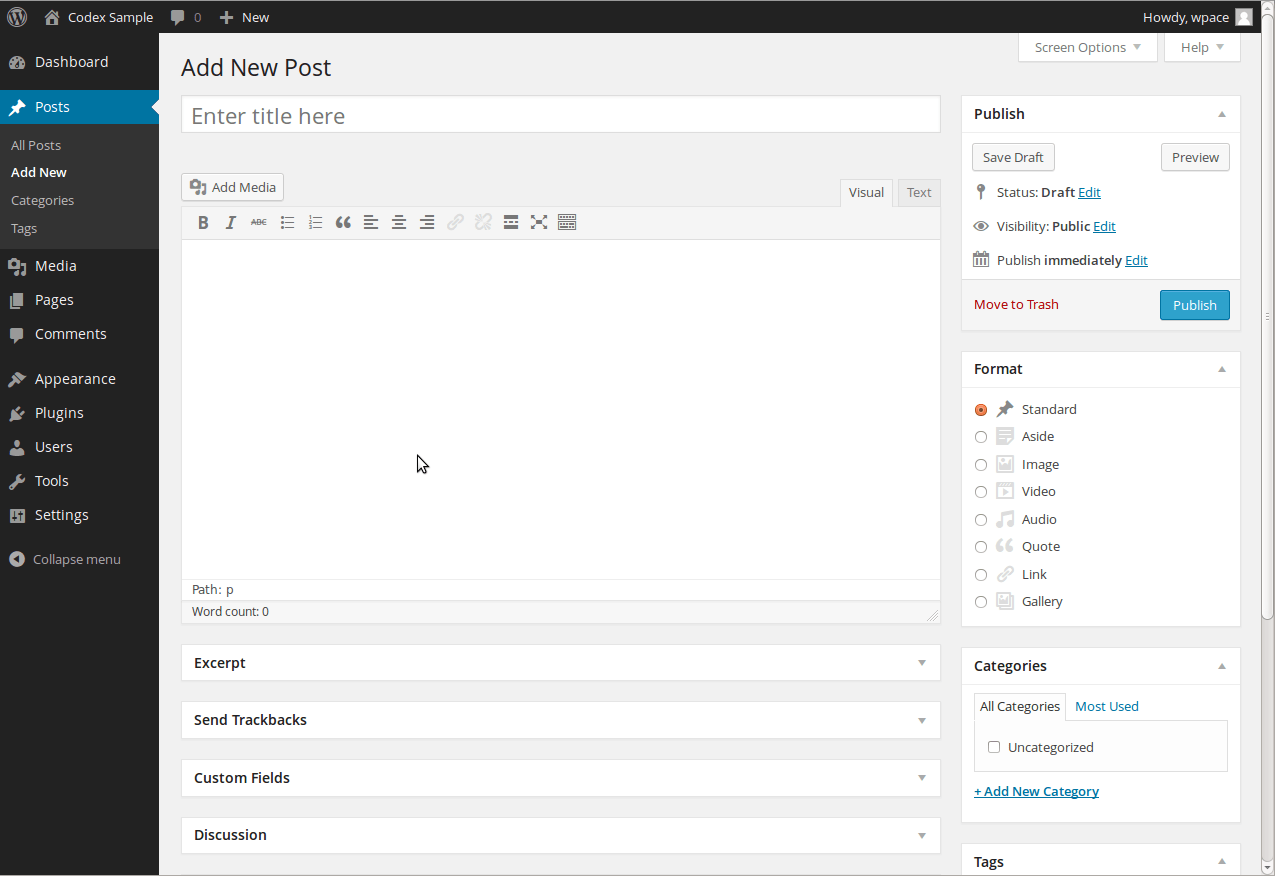
\includegraphics[width=1\textwidth]{./img/wordpress_new_post.png}
    \caption{Tworzenie nowego wpisu w systemie Wordpress}
    \label{wordpressNewPost}
\end{figure}

\FloatBarrier

% https://wordpress.stackexchange.com/questions/158742/add-custom-objects-entities-to-wordpress
% https://developer.wordpress.org/reference/functions/register_post_type/

Pisanie własnych zapytań SQL jest możliwe, ale podobnie jak definiowanie
niestandardowych typów, domyślnie nie posiada interfejsu. W celu napisania
własnego zapytania, trzeba to zrobić z poziomu PHP, lub zainstalować wtyczkę
umożliwiającą pisanie własnych zapytań z panelu administratora.

W wersji 5.0 Wordpress, dodano nowy edytor ``Gutenberg'' pozwalający na
tworzenie postów opartych o bloki. Jest to mniej skomplikowana alternatywa dla
stosowanych do tej pory tzw. ``online rich-text editor''. Edytory blokowe
pozwalają na tworzenie wpisów składających się z bloków. Blok może zawierać
tekst lub media. Bloki tekstowe mogą reprezentować nagłówek lub paragraf, a
paragrafy mogą mieć fragmenty z ograniczonym stylizowaniem jak na przykład
pogrubieniem czcionki. Wpisy w formie bloków są łatwiejsze w przechowywaniu i
wyświetlaniu na stronie HTML. Nie jest konieczne na przykład parsowanie treści
wpisów, żeby wydobyć informacje o zdjęciach, jakie zostały zamieszczone we
wpisie.

Wpisy oparte o bloki mogą być wygodnie tworzone w dużo prostszych edytorach.
Zmniejsza to potrzebę stosowania skomplikowanych systemów CMS do zarządzania
treścią.

Podsumowując, Wordpress to oprogramowanie, które dobrze spełnia potrzeby autora
bloga. Znaczną zaletą systemu Wordpress jest ekosystem wtyczek pozwalających na
rozwiązanie większości problemów związanych z zarządzaniem danymi.

System Wordpress domyślnie znacznie ogranicza możliwości administratora. W celu
wykonywania niestandardowych operacji na bazie danych, administrator musi
polegać na wtyczkach, lub samemu napisać umożliwiające to wtyczki. Zwiększa to
znacznie wymagania wiedzy wobec administratora.

Pomimo tego, możliwe jest skonfigurowanie systemu Wordpress w taki sposób, żeby
spełniał wszystkie funkcje przygotowanego w ramach tej pracy systemu. Taka
konfiguracja byłaby jednak mniej stabilna od sytemu, który powstawał w celu
spełnienia tych celów. Niezbędne byłoby poleganie na dużej ilości wtyczek, lub
napisanie tych wtyczek samemu, co może być bardziej skomplikowane, niż napisanie
systemu backend spełniającego potrzeby jednej strony internetowej.

(TODO: cite Wordpress bible)

\subsection{Strapi}

Strapi to system Headless CMS. Nie posiada on interfejsu użytkownika. Dane
wprowadzane do systemu są pobierane za pomocą API REST. Domyślne API ma
ograniczoną funkcjonalność. Pobieranie danych z CMS jest ograniczone do
pobierania wszystkich wpisów danego typu, lub jednego wpisu, ale tylko po id.

Strapi umożliwia tworzenie własnych punktów końcowych. Administrator może ustawić
ścieżkę i funkcję, która obsłuży zapytania na daną ścieżkę. Nie da się jednak
zrobić tego w panelu administratora. Administrator chcąc stworzyć niestandardowy
punkt końcowy musi sam napisać funkcje, które obsłużą zapytania w języku
JavaScript. Jest to porównywalnie skomplikowane do napisania kontrolera w
zwykłej aplikacji internetowej. Ponadto, na administratora są nałożone pewne
ograniczenia. System Strapi wspiera wiele baz danych, w tym MongoDB, która nie
wspiera SQL. Z tego powodu, nie jest możliwe pisanie natywnych zapytań do bazy
danych. Do operacji na bazie danych Strapi udostępnia ``query engine''. Jest to
biblioteka do operacji na bazie danych z poziomu języka JavaScript. API
udostępnione programistom przez ``query engine'' jest znacznie ograniczone w
porównaniu do natywnego SQL. Nie można używać funkcji specyficznych do wybranej
bazy danych. Operacje są ograniczone do prostych zapytań CRUD.

Strapi umożliwia operowanie na danych za pomocą GraphQL. Ta opcja pozwala na
pobieranie konkretnych danych o wpisie zamiast całości informacji. W celu
pobierania niestandardowych informacji, wymagane jest pisanie własnych
``resolwerów''. Pisanie resolwerów przypomina pisanie funkcji obsługującej
zapytania do REST API. Wymaga pisania kodu źródłowego w języku JavaScript.

Podsumowując, Strapi jest dobrym wyborem, jeśli potrzebny jest system CMS
pozwalający na bardziej złożone od CRUD operacje na danych. Niezbędne będzie
jednak pisanie własnych funkcji obsługujących zapytania z wykorzystaniem
ograniczonego API do operacji na bazie danych.

Znacznym minusem Strapi są duże wymagania wobec sprzętu. Minimalna ilość pamięci
to 2GB \cite{StrapiDeployment}. Nie jest to problem dla przedsiębiorstw, ale
może to zwiększyć koszty osób zarządzających mniejszymi stronami internetowymi.

% https://docs.strapi.io/developer-docs/latest/setup-deployment-guides/deployment.html

\subsection{PostgREST}

PostgREST nie jest systemem CMS. Twórcy definiują ten program, jako samodzielny
serwer internetowy, który przemienia bazę danych Postgres w API REST
\cite{PostgrestDefinition}. Mimo tego, PostgREST spełnia dużą część założeń tej
pracy dyplomowej.

PostgREST jest przeznaczony do pracy tylko z bazą danych PostgreSQL. Dzięki
takiej specjalizacji, umożliwia on korzystanie z funkcji specyficznych dla bazy
danych PostgreSQL. Umożliwia wyłuskiwanie danych z kolumn o typie \texttt{json}
\cite{PostgrestJson} i korzystanie z funkcji full-text search \cite{PostgrestFts}.

Minusem serwera PostgREST jest to, że zapytania SQL są kodowane w parametrach
zapytania HTTP, co zmniejsza czytelność zapytań SQL. Można to zauważyć w
przykładowym zapytaniu z dokumentacji PostgREST pobierającym dane z wielu tabel:

\begin{verbatim}
GET /films?select=title,actors!inner(first_name,last_name)
        &actors.first_name=eq.Jehanne HTTP/1.1
\end{verbatim}

\noindent Powinno zwrócić dane JSON:

\begin{verbatim}
[{
    "title": "The Haunted Castle",
    "actors": [{
        "first_name": "Jehanne",
        "last_name": "d'Alcy"
    }]
}]
\end{verbatim}

Podsumowując, jeśli aplikacja będzie wymagała dużej ilości niestandardowych
operacji na bazie danych, PostgREST z dodatkiem prostej aplikacji serwerowej
jest dobrym wyborem, jeśli nie potrzeba panelu administratora. Jest to jedyne
omawiane do tej pory narzędzie, które nie ogranicza w większym stopniu
możliwości operowania na bazie danych.

\subsection{Podsumowanie}

Podsumowując, można zauważyć, że na rynku nie ma popularnego narzędzia
spełniającego założenia pracy. Istnieje wiele narzędzi, które można dostosować
do założeń pracy, ale takie zastosowanie nie jest zamierzone przez twórców, lub
wymaga pisania kodu poza zapytaniami SQL.
